\documentclass{article}


% Packages
\usepackage[utf8]{inputenc} % For Norwegian letters
\usepackage{tabulary} % For nice tables
\usepackage{graphicx}
\usepackage{hyperref}
\usepackage{float}
\usepackage{listings}

% Config
\setlength{\parindent}{0pt}
\setlength{\parskip}{1em}

\begin{document}

% Title
\title{\textbf{Module 4} \\ IT3105}
\author{Simon Borøy-Johnsen \\ MTDT}
\date{\today}
\maketitle
% End Title


% Content
\section{Structure}
The game board is represented as a two-dimensional array of Cell objects. A Cell object has a position, a value, and a boolean value telling whether the cell has been merged or not (this value is set to False before each player move). The cell value is given as the exponent over 2 in the cell ($1024 = 2^{10} \rightarrow value=10$).

Making a move is done by iterating through all cells in the grid, staring from the edge the cells are moving towards. For each cell, its nearest non-empty neighbour is checked. If the value of the neighbour matches the cell, they are merged. If not, the cell moves to the farthest empty cell in the moving direction. By starting the iteration from where the cells are going, the game board can be changed on the go during the iteration.

\section{Expectimax}
I used expectimax with dynamic depth in my solution.

The depth is chosen before each player move;
\begin{lstlisting}
def get_depth():
    if number_of_empty_cells > 3:
        return 1
    elif number_of_empty_cells > 1:
        return 2
    else:
        return 3
\end{lstlisting}
I found this choice of depth to be sufficient in order to achieve 2048. It is very shallow compared to other implementations, but it yields consistent results good enough to achieve the top score for this assignment.

My expectimax implementation consists of two main components (Python functions);
\begin{itemize}
    \item evaluate\_player\_move(depth): This function returns the expected score (heuristic value) of the current game board. For the four different directions to make a move, the outcome of making the move is evaluated. If the depth is 0, whatever move yields the highest score is returned. If not, the function evaluate\_computer\_move is run (with same depth), and whatever move yields the highest expected score is returned.
    \item evaluate\_computer\_move(depth): In this function, all possible computer moves are simulated (a computer move is just spawning a 2 or 4, with probabilities 0.9 and 0.1, respectively, at a random empty cell). For every possible computer move, the evaluate\_player\_move (with one less depth) is run. All the results of running evaluate\_player\_move are weighted, and the mean is returned.
\end{itemize}

The two functions combined create a recursive search algorithm. The algorithm evaluates the next (player) move, and the $n$ next moves thereafter, with $n$ being the depth of the search.

For each time the player is about to make a move, each of the four possible directions to move are evaluated. If the move is valid (changes state), all possible computer moves following it are simulated. The algorithm restart from each of the simulated states.

\section{Heuristic}
I used a rather simple heuristic function in my implementation of the 2048 solver.

The board is organized into a "path", following the pattern in figure \hyperref[fig:path]{[\ref*{fig:path}]}.
\begin{figure}[H]
	\centering	
	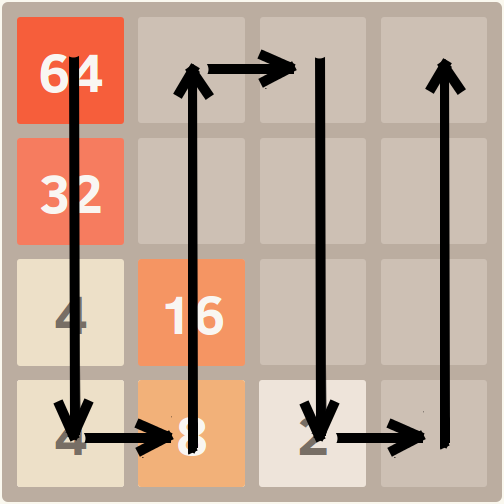
\includegraphics[width=0.5\textwidth]{path.png}
	\caption{Path pattern}
	\label{fig:path}
\end{figure}
Each cell in the path is given a label, $p_n$, with $p_0$ being the upper left cell, $p_1$ the one below, and so on all the way to $p_{15}$ in the upper right corner.

The score (heuristic value) of the board is then calculated using this formula;
\begin{equation}
	\sum\limits_{n=0}^{15}value(p_n)*r^n
\end{equation}
where $value(p_n)$ is the value at cell $p_n$, and $r$ is a constant in the range $(0, 1)$ (set to 0.25 during the demo session).

This enforces a monotonic decreasing order along the path, as $r^n$ decreases for each step. The AI will therefore do what it can to get the larger values as close to the start of the path as possible. Since the AI tries to put the highest values as early in the path as possible, it will gather them, allowing them to merge together to form even higher values.

Example: With $r=0.25$, a 512 in cell $p_n$ would yield four times as much to the score as it would in cell $p_{n+1}$. A 512 in cell $p_n$ would be equivalent to a 2048 in cell $p_{n+1}$.

% End content

\end{document}
